\documentclass[11pt]{article}
\usepackage[margin=1in]{geometry}
\usepackage{graphicx}
\usepackage{microtype}
\usepackage{verbatim}
\usepackage{amsmath}
\usepackage{nicefrac}
\usepackage[colorlinks=false, pdfborder={0,0,0}, hidelinks]{hyperref}

\begin{document}
\title{Conveyor Belt \& Sunlight Monitoring\\Embedded System Design, Lab 3}
\date{October 1, 2015}
\author{Ben Lorenzetti}

\maketitle
\tableofcontents
\clearpage

\section{Objectives and Problem Descriptions}

\section{Procedure}

\subsection{Conveyor Belt Controller}

The circuit for the conveyor belt controller is shown in figure \ref{conveyor-circuit}.
There are two LEDs and two pushbuttons.
A green LED indicates if the phototransistor is detecting a box in the line of sight.
A red LED is used as a blinking alarm in case of jam.
The two pushbuttons are for indicating that a jam has been manually cleared
and for indicating the end of a shift.

\begin{figure}[h!]
\centering
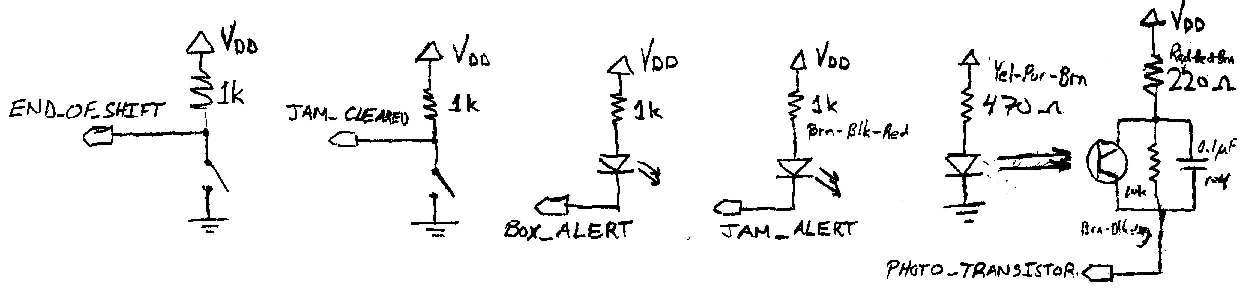
\includegraphics[width=.9\textwidth]{conveyor-circuit.pdf}
\caption{Conveyor Belt Controller Circuit}
\label{conveyor-circuit}
\end{figure}

The conveyor belt specifications had a lot of requirements, including
status upon reset and non-volatile memory. My approach to dealing with
all of these requirements was to create a state diagram and a main loop
model where the main loop has the ability to change states once per loop
and takes actions based on the current state.

The program flow is shown in the implementation flowchart in figure
\ref{conveyor-flowchart} and the transistions for the state variable
are shown in figure \ref{conveyor-state-diagram}. I think these diagrams
show my approach to the problem more concisely than could be explained
in words.

\begin{figure}[h!]
\centering
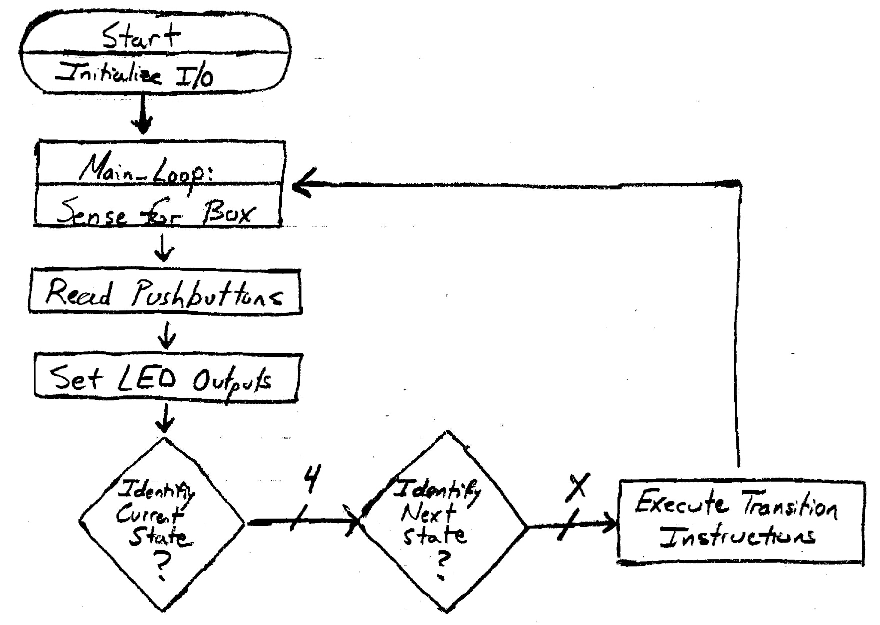
\includegraphics[width=.5\textwidth]{conveyor-flowchart.pdf}
\caption{Conveyor Belt Implementation Flowchart}
\label{conveyor-flowchart}
\end{figure}

\begin{figure}[h!]
\centering
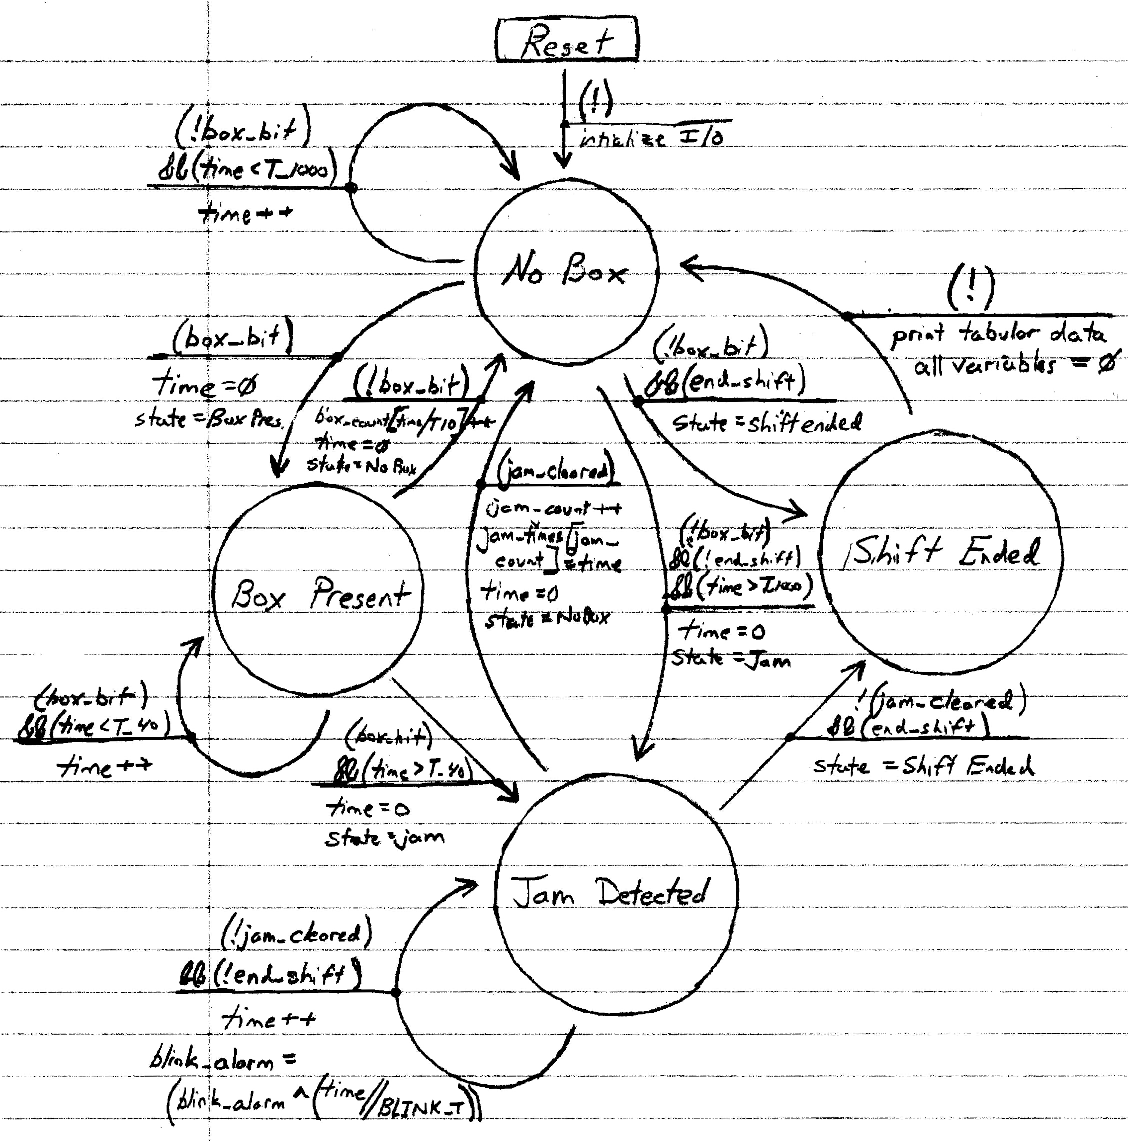
\includegraphics[width=.8\textwidth]{conveyor-state-diagram.pdf}
\caption{State Diagram for Conveyor Belt Controller}
\label{conveyor-state-diagram}
\end{figure}

\clearpage
\subsection{Sunlight on Planet Alpha Controller}

The circuit for the sunlight sensor is shown in figure \ref{sunshine-circuit}.
An LED is used in reverse bias as a photosensor: greater light intensity
causes an increase in the reverse bias leakage current.
\texttt{RCTIME} can be used without a capacitor because the diode
and an appropriate junction capacitance for the 2$\mu$s time resolution
of the microcontroller. The 220 $\Omega$ resistor limits the charging current
from damaging the microcontroller.

\begin{figure}[h!]
\centering
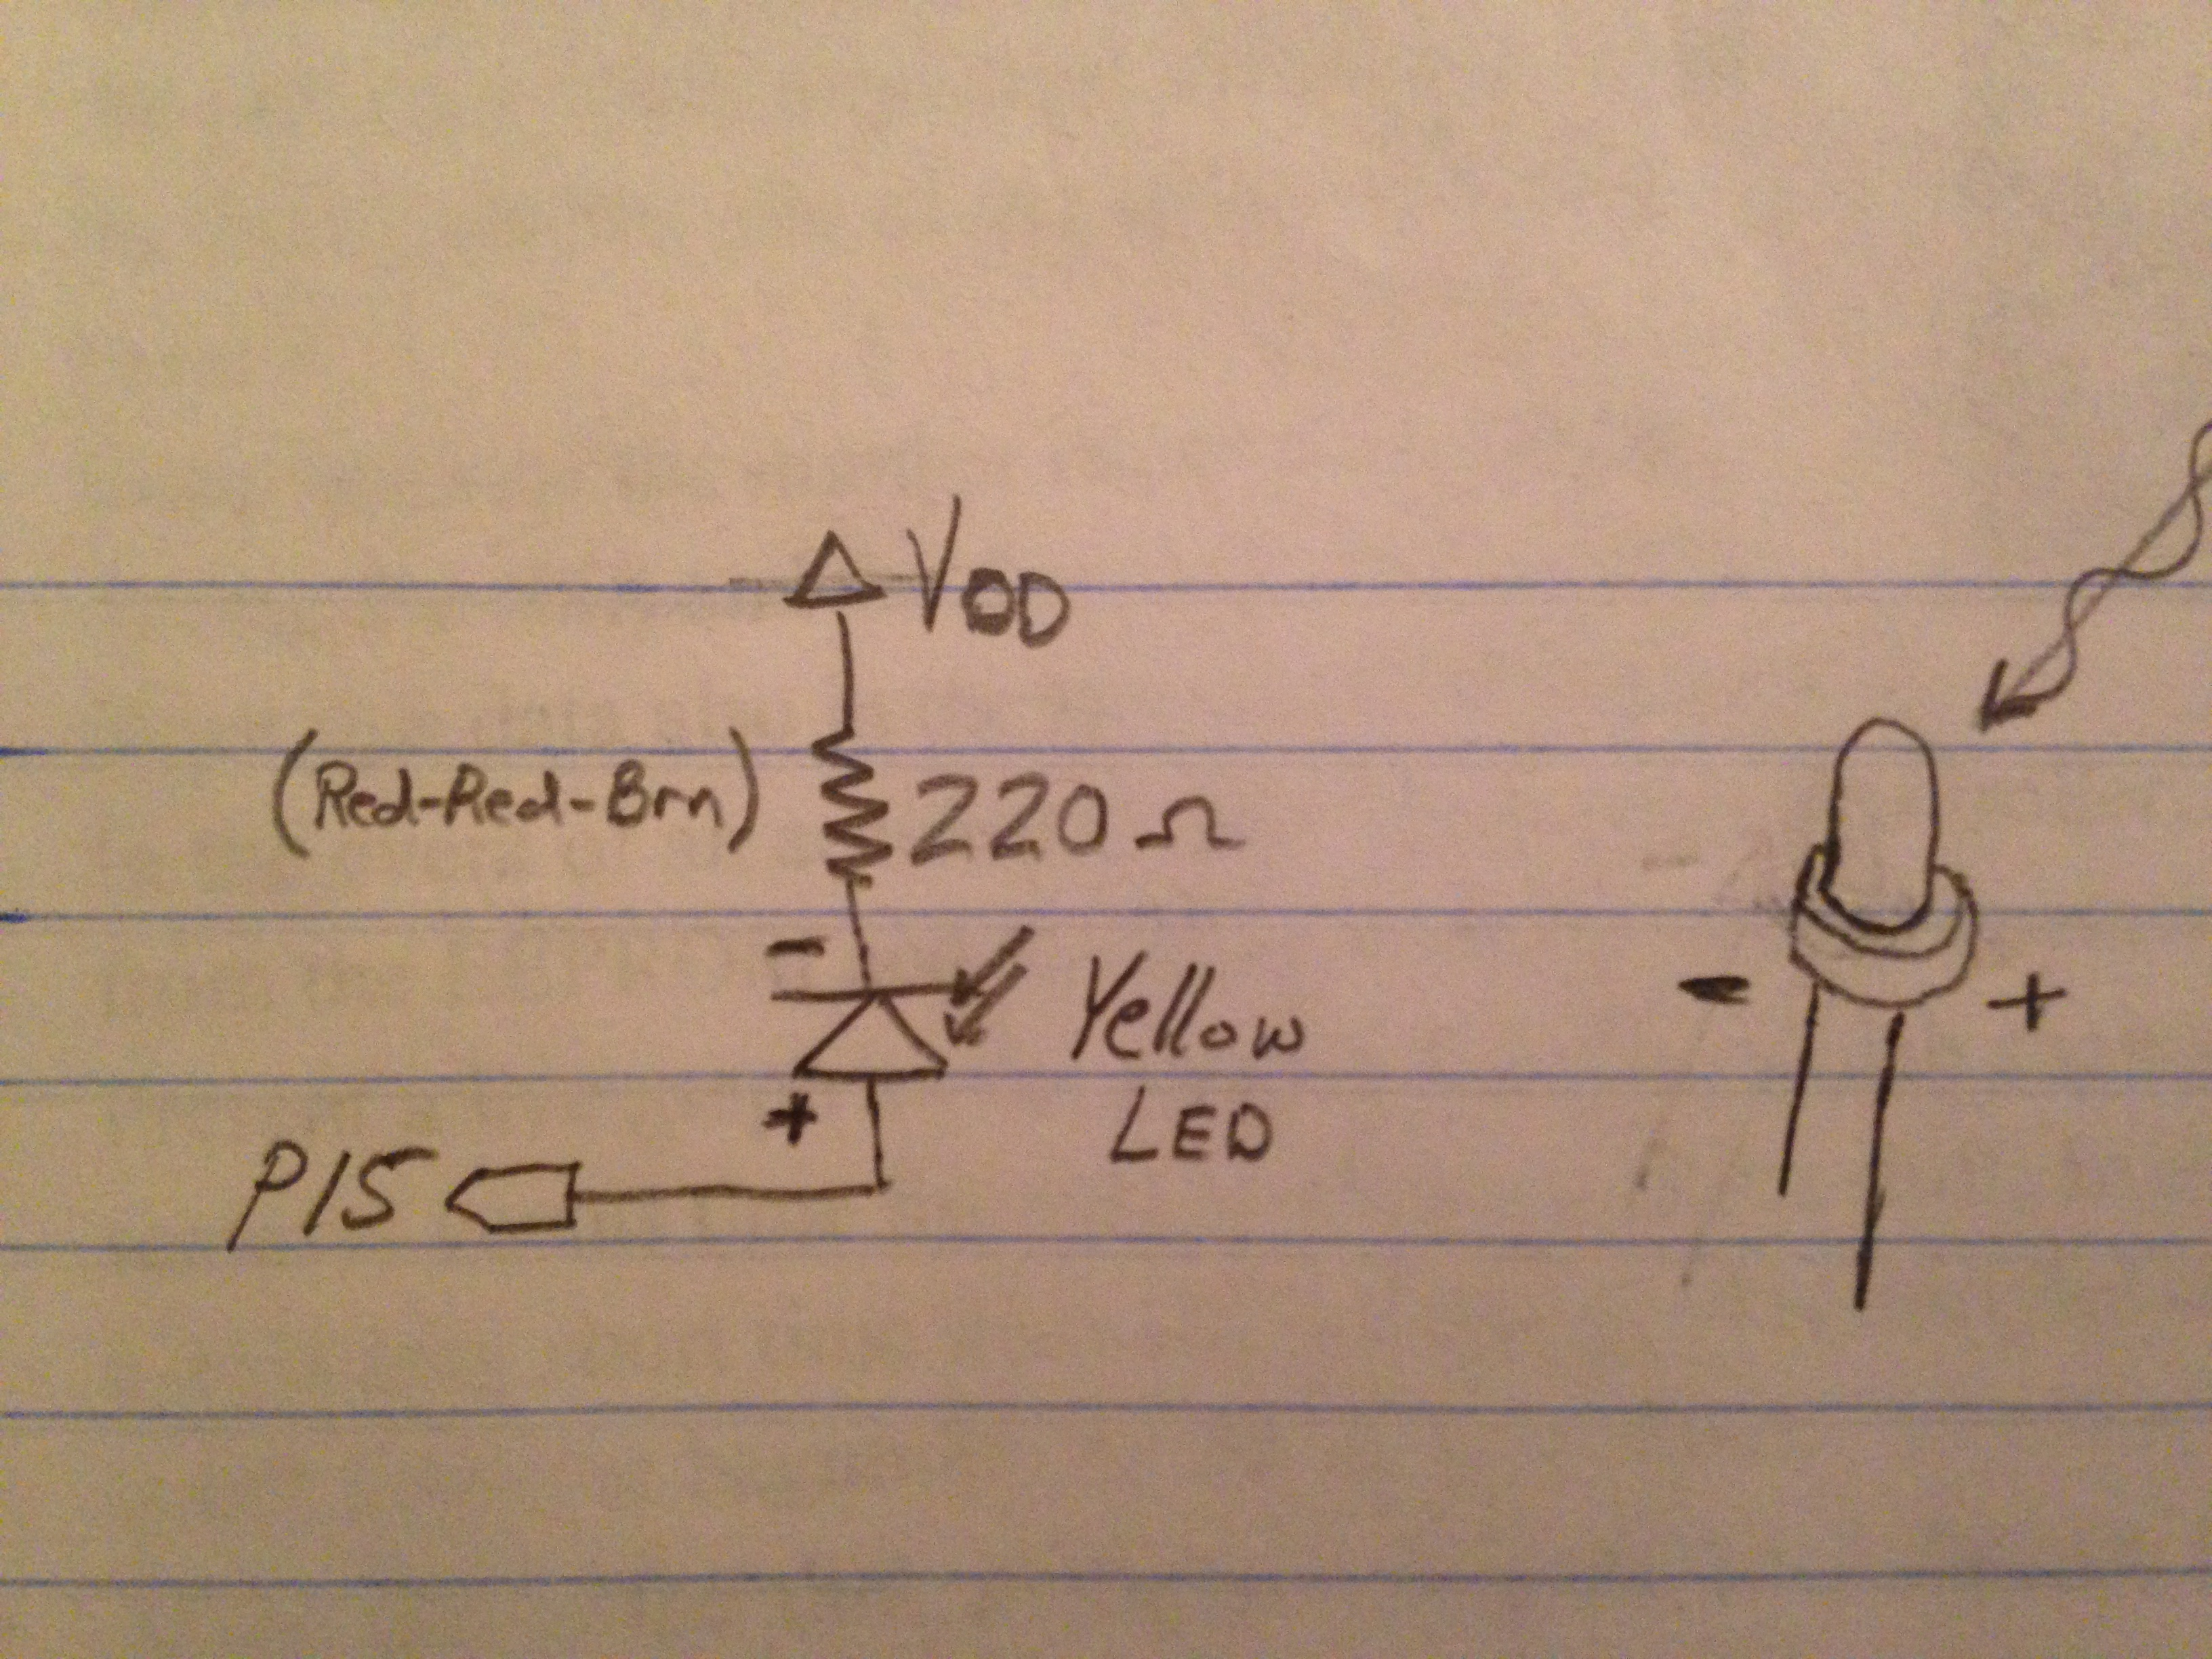
\includegraphics[width=.45\textwidth]{sunshine-circuit.jpg}
\caption{Sunlight Sensing Circuit}
\label{sunshine-circuit}
\end{figure}

The programming for the sunlight sensing controller was also easy.
Upon reset, the controller attempts to dump all its recorded data to
a Debug channel and also prompts the user the current data should
be discarded.
Importantly, the default is no so that data is not lost if the Debug connection is not active.

Then, the microcontroller takes one measurement every 15 minutes and saves
the data to EEPROM. In between it sleeps to conserve power.
The program flowchart is shown in figure \ref{sunshine-flowchart}.

\begin{figure}[h!]
\centering
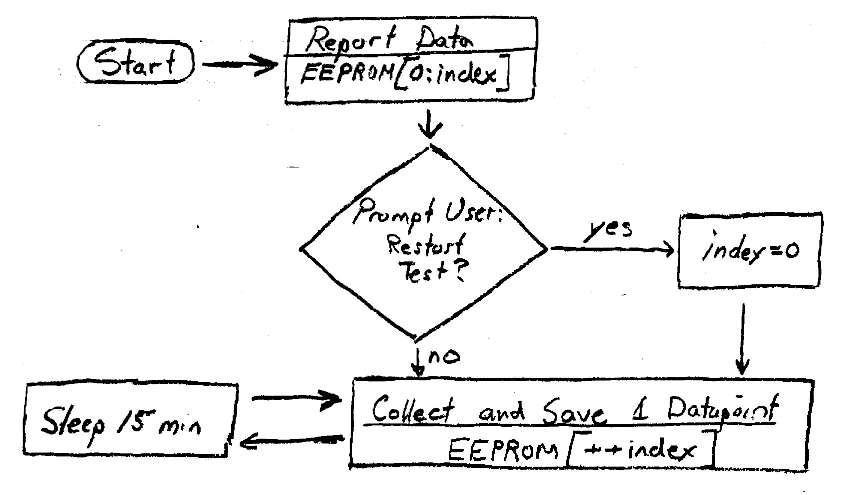
\includegraphics[width=.65\textwidth]{sunshine-flowchart.pdf}
\caption{Sunlight on Planet Alpha Implementation Flowchart}
\label{sunshine-flowchart}
\end{figure}

\section{Expected Results}

For the conveyor controller, I expected results that matched the specifications--minus
probably not having the timing for the main loop correct (\texttt{T\_10\_INCHES}).

For the sunlight data, a low number indicates strong light and an
high number indicates dark conditions.

\section{Experiment and Design Revisions}

The conveyor circuit worked as expected, using R and C values from the prior lab.

For the sunlight sensor, I ran several test experiments to get the best divisor term
to ensure the data was always withing 0-255. One interesting thing I noted was
that if \texttt{RCTIME} timed out (i.e. if the room was completely dark), then
the time returned was zero instead of the maxium $2^{16}-1$.

\section{Observations}

The sunlight sensor was placed in the window of my room for \~ 24 hours.
Afterwards, I retrieved the data with the Debug terminal and imported it
into excel as a space-separated list. I changed all zero values to 255 manually
based on what I learned in experimentation/design revisions.

Finally, I plotted the inverse of the times measured to show sunlight
intensity over the course of the day. This is shown in figure \ref{ambient-lighting-results}.

\begin{figure}[h!]
\centering
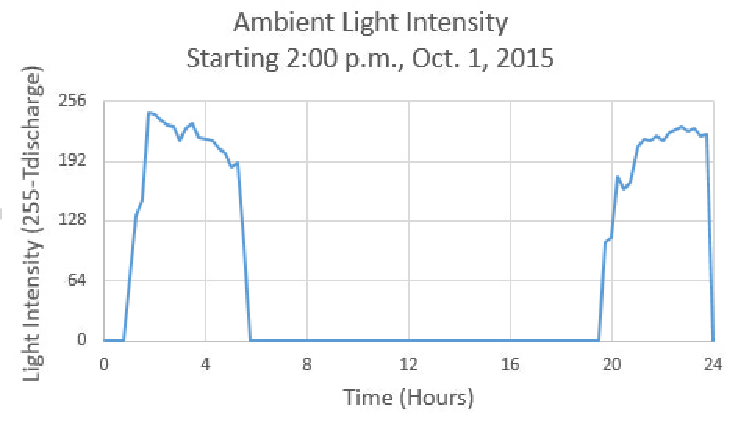
\includegraphics[width=.7\textwidth]{ambient-lighting-results.pdf}
\caption{Ambient Lighting of My Bedroom Window}
\label{ambient-lighting-results}
\end{figure}

\clearpage
\section{Implementation Code}

\subsection{Converyor Belt}
\begingroup
\fontsize{10pt}{12pt}
\verbatiminput{Conveyor-Belt.bs2}
\endgroup

\clearpage
\subsection{Sunshine Monitoring}
\begingroup
\fontsize{10pt}{12pt}
\verbatiminput{Sunshine-on-Planet-Alpha.bs2}
\endgroup

\end{document}